% !TEX root = ../main.tex
\section{The Survey}\label{sec:survey}
  
  The problem with analyzing passwords is that you need to actually have passwords to analyze. The majority of published research on passwords are often using passwords for leakage or getting passwords distributed from legal sources. Looking at the Android lock pattern there exists no distributed sources, and all lock patterns are only stored locally on each device. 

  People working with security are striving to teach people about security, and one of the rules everyone probably know about is that you should never share a password because it is a secret you should keep to yourself. In this research I have to be a hypocrite and do the opposite; I need to ask people to share their secrets in the name of science. 

  This section will include a detailed description of how the custom made survey was created and how it works. The survey is created for collecting Android Pattern Locks and other background data from the users on mobile devices. 

  \subsection{Requirements}

    When coping with the difficulties with collecting data it is important to define requirements for the survey application. This section will not go through a predefines list of requirements, rather elaborate and discuss the requirements in general to be able to explain its importance.

    \subsubsection*{One way Communication}
      The survey will be a online application, meaning that this is the only way I as a researcher will be able to communicate with the respondents. It is therefore important how the application are communicating with the respondents.
      The survey will contain a number of questions to be answered by the respondents. The hard part is to adapt the suitable amount of questions. If the survey takes too long time to answer I will probably loose respondents.
      When sending out the survey I have no control over who will participate, so people might come from different cultures and countries. The survey will be written in english, but there is a chance that there persons entering the survey not speaking english very well. Instead of using too much words it is preferable to use icons and illustrations. This is not just beneficial for respondents not talking english. 
      The words used in the questions have to be carefully selected considering that all respondents have a different background. It should be avoided using academic and technical words that I cannot ensure that everyone can understand. It should also be considered that some respondents do not know what Android, locking mechanism, or pattern lock is. It should be visualized, explained and support practice for the respondents needing it. It is not disired that any respondents are feeling stupid nor insecure when participating. 

      % - ordbruk: korte setninger for at folk skal gidde å lese.
      % - ordbruk: spørsmålene må være formulert på en måte slik at alle forstår (unngå tekniske uttrykk)
      % - Unngå lange setninger
      % - Unngå at personer føler seg utrygge eller dumme fordi de ikke kan svare.  (treningsmodus og valgalernativer som fører personen ut av en ukomfertabel sone, men samtidig gi data som kan brukes. )
      % - Naturlig valg å bruke engelsk, men ikke alle kan engelsk --> kommuniserer spørsmålet med ikoner. 
      % - Cross-cultural requirements
      % - Kan ikke anta at alle vet hva låsemønster og android er

    \subsubsection*{Trustworthiness}
      When respondents opens the survey they should be able to see who are asking them to participate. Is is reasonable to provide contact information and information about myself so the participants can read and see who I am. The survey should be a subdomain on my personal domain marteloge.no to gain trustworthiness. Linking to my personal page and contact information should be required.
      The contact information are also important in terms of ownership of data. Who are reading the data and how is it handled? It should be clearly stated that the information collected are only available to the research group containing myself, my supervisor, and my co-supervisor.

      The visual appearance is an important part of the thrustwortiness of the survey. If you put a pink webpage that is visual appealing next to a webpage using only dark colors. Colors tell more than you probably would think in the first place.

      % - OBS: må her ref til forskning!
      % - Tilgjengeliggjøre meg selv via nettside og kontaktinformasjon. Det er virktig å vise at det kommer fra en seriøs kilde og det er viktig å vise hvem som spør om hjelp. Må fremstå som pålitelig og lite skummel. 
      % - Fargebruk og bilder må virke lite skumle. 
      % - Lage et eksempel på et bilde med mørke farger og et med lyse farger for å hvise at det har mye å si på hvordan man kommuniserer ut til bruker. 
      % - Vise til hvem som mottar og behandler data

    \subsubsection*{Technical device and environment of use}
      When collecting data the environment should be considered because it can impact the data or introduce bias. Looking at the Android Unlock Pattern it is often used on mobile devices, both tablet and smartphones. When looking at different human properties and characteristics of mobile devices, tablets should be divided into two different environments of use. {\it First}, the tablet are often used in different settings than a smartphone that a user often carry and use every day. {\it Second}, the physical interaction are often diffrent. A smartphoene are small and can be intereacted with using one hand. When collecing data I want to capture specific characteristics that will be different on a smartphone and a tablet. It is therefore desirable to only collect data on a smartphone where it is most rapidly used. It does not mean that patterns on tablets are not interesting, but to ensure what environment the survey are used for analysis purposes. 

      A decision to only deploying the survey on smartphoens sets high requirements to the usability. It is not a easy job to design a survey that will work on small devices, but there is also an technical part of this to fit the design to all various screen sizes. 

      The choice to have a online survey can both give positive and negative outcomes. When only using a online survey I do not have any control of who have answered and I can not be there observing or asking questions. The other choice of only using smartphones do also impact what kind of users that will answer. By only using smartphones I will neither be able to reach people not in possession of a smartphone. One positive thunk with going online is that I do not know who will answer the survey. The survey will therefore be anonymous. Most of the people in my network that I am able to reach in person do almost have the same age and the background. Going online helps me reach people outside where I live and outside my own network.

      % - Andorid brukes bare på små enheter
      % - Vil ikke samle inn data som ikke er generert fra det miljøet det vanligvis brukes. Mulig man kan få flere svar med å samle inn data på desktop, men dataen mister credability. Basert på analysen av hvilke egenskaper som skal inkluderes kan ikke de anlyseres om spørreundersøkelsen ikke blir tatt på en mobil enhet. 
      % - Setter høye krav til kontroll
      % - Setter høye krav til brukergrensesnitt
      % - Utelukker muligens noen brukere som ikke eier en smarttelefon, men kan anta disse som ikke relevante for sample siden de ikke eier teknisk utstyr som er nødvendig. 
      % - Mister kontroll på hvem som svarer, men styrker også anonymitet fordi jeg ikke har mulighet til å sjekke hvem som svarer.

    \subsubsection*{Complexity and length}
      Because of the decision of using the technical environment of the smartphone it do impact the complexity and length of the survey. The smartphone have a limited ability for interaction where the small touch screen are the only interaction available. To get people to complete the survey it need to have well picked questions with a short and concise formulation, and the questions should be easy to answer. It may be needed to shorten the number of questions because of the chosen environment. There will always be a risk of people not completing the survey; each questions should carefully be prioritized after its importance for the study. It is better to get some data than nothing at all. Each answer for each question should be stored after the submission of each question. 

      The complexity do also include how people will understand the questions. Computer security are for many people something unknown. It should therefore provide the information needed to complete the survey and it should be avoided using complex academic and technical terms that are not common to use. A situation where a person do not understand what is asked for should be avoided. The feeling of feeling stupid because you do not understand what to answer or do will probably result in the participant leaving the survey. People might having less understanding of the technical part are probably older adults that I fear are hard to reach in the first place.

      % - Hvis undersøkelsen blir for lang er det fare for at mange vil avbryte undersøkelsen før den er ferdig
      % - Selv om man kommer med prevantive tiltak mot lang undersøkelse er det viktig å prioritere spørsmålene etter prioritert rekkefølge (viktighet av spørsmål).
      % - Det er veldig viktig at ingen føler seg dumme når de gjennomgår spørreundersøkelsen. Det kan komme tilfeller der personer som ikke har brukt løsemønster vil svare. Det er defor lagt til treningsmodus for at alle skal føle mestring og unngå frustrasjon.
      % - Som nevnt på språk og kommunikasjon er det viktig at spørsmålene er lette og korte der man også unngår kompliserte ord og tunge faguttrykk.
      % - Lengde og data nødvendig for å kunne analysere data

    \subsubsection*{Visual appearance and psychology}

      % - Å li bedt om å lage mønster/password kan for mange virke som en avskrekkende ting. Det er derfor virkig å utnytte psykologien! Bruk farger som virker imøtekommende og som ikke forbindes med noe farlig. 
      % - Ikoner kan også hjelpe å gi undersøkelsen et "barnslig" preg som også gjør at det virker mindre skummelt
      % - Viktig å vise hvem jeg er og at jeg kan stoles på. Dette er nevnt tidligere, men vis tydelig bilde slik at personer får tiltro. Hjemmesiden min er laget rosa fordi 1) det faktisk representerer meg 2) det virker ikke skummelt.
      % - Gjøre meg tilgjengelig.
      % - Finnes det noe fargeteori som kan refereres til?
      % - Finnes det noe forskning på hva man må gjøre når man lager spørreundersøkelse?
      % - Spørsmålnr og antall spørsmål igjen. 
      % - Tradisjonelle spørreundersøkelser på mobil blir ofte tatt dårlig imot fordi det er tungvindt å svare på. Jeg ønsker å gi et personer et overasket øyeblikk og deretter ønske å dele den videre fordi den var anderledes. Spille på sosiale aspekter for å få spredt den og bygge thrustworthyness. Det er ingen som vil dele en dårlig spørreundersøkelse med mindre det er din beste venn som spør. 
      % - Må kommunisere at dette er sikkert. det går også innom aspektet med psykologi. Man må visuelt se at det føles sikkert. Feks å se HTTPS er et enkelt inngrep som kan gjøres.

    \subsubsection*{Navigation}
      Using a smartphone sets requirements to the navigation in the survey. It is desireable to reduce the number of clicks used to complete the survey. The navigation should in some way be automaic when the participant select their answer. The selected answer should be clearly visualised and the navigation to the next question should go automatic. To signalize the number of questions left it will be added a navigation bar to show the progress. 

      % - Når man jobber på en mobil er det viktig at det går rask og smooth.
      % - Navigasjon er vanskelig på mobil fordi det eneste man verktøyet man han er en touch skjerm for å interaksjon med mobilen. Det skal gå fort men samtidig være lett.
      % - Det er fort å minste brukeren om det går for fort i svingene. Det bør tydelig vise brukeren hvor den er, hvor den var og brukeren bør for få en følelse av hva som skjer når man trykker eller interagerer med elementer. 
      % - Må bygge tydelige tilbakemeldinger til bruker underveis i navigasjon

    \subsubsection*{Security}
      Since the survey are anonymous, the communication should be transfered over an encrypted channel using SSL. It provide actual security and anonymity, but it also adds to the visual part of the security. Using SSL provides the secure HTTP (HTTPS) in the navigation bar helping also to build upon the trustworthiness of the survey.
      On the backed of the application, all logging and traces of the users should not be stored. The only data stored should be the answers provided by the participants. 
      Other security measures should also be provided and the survey should be reviewed by someone with a high competence in computer security. It is not desired to loose any data or a situation where someone are able to steal the data in any terms.
      If any cookies are used, it should be clearly stated in the introduction. The introduction should also include a description of any information about security of the application in interest of the participant.
      % - Spørreundersøkelsen håndterer data som ikke bør kunne avlyttes. 
      % - Den tekniske løsningen bør gå over krytert kommunikasjon og den bør på ingen måte logge data som kan brukes til å spore tilbake brukeren.


	\subsection{Layout and Structure}

    The layout and design was first drafted in my specialization project in 2014. The wireframes can be found in Appendix \ref{ap:wireframes}. Since the first drafts was made, the technical implementation and redesign have been carried out. 

    \subsubsection{Introduction}
      When entering the survey application on a smartphone, all users will see an introduction with information about the survey, the research, and the author. The survey starts will not start collecting any data before a visitor decides to start the survey. When the visitor clicks on the green button, "start survey", the visitor becomes a participant in the study and will be sent to the rules of the pattern lock. It is important to give a brief explanation to users not familiar with the pattern lock, but it is not desirable to give too detailed information that can cause bias in the data. Figure \ref{fig:startscreen} and Figure \ref{fig:ALPintroduction} are showing the introduction to the survey and the introduction to the Android Pattern Lock respectively. In Figure \ref{fig:ALPintroduction} the participant have two choices; either enter the training mode or skip the training mode. If the respondent have never used the Android Pattern Lock before, there is added a training mode to avoid an uncomfortable situation where the user gets the feeling that they are tested in something they do not know how work. The training mode is an opportunity for the participant to play with the pattern without feeling any pressure to perform. This is also an opportunity for me to collect data from this.

      I as researcher believe that the patterns created in the training mode will be as real and valid as the other main pattern types collected. The reason for this is that people might tend to create the first patterns that pops into their mind without thinking too much about what they actually are creating. As far as this research know about there are not published any research on how people think when they are asked to create a password or asked by someone to give away a password. Think about the situation where you ask a person "Are you stupid?". By testing this question on some of my friends they just looked at me with a weird face and answered "NO?!". I believe that asking people to "give away" a password or pattern will give the same effect; people tend to overachieve when giving away a password or pattern just to prove that they are not stupid. When people are under pressure to perform, and when the outcome are related to how people might be judging you, you would probably do anything to put yourself into a position where you look good. When someone are asking about their password, and they know it is bad, they actually realize that they might are under the category stupid because they do know it is a bad choice but they do not want to do anything about it for many reasons. In the related work it was stated that the reason for using a bad password, or not using a password at all, was because the overhead in time used to type that complex long password and the hard work of actually remembering the password. 

      In the training mode I try to give a relaxed situation where people get the feeling of not being tested. Later when people are asked to create 3 different patterns for three different security levels, I believe that people might get the feeling of being tested and would might create a pattern that normally not would appear "in the wild". Figure \ref{fig:trainingmode} shows the training mode. This view has a feedback mode showing if a pattern is valid or not and the participant can try to create as many patterns as they like. To continue the survey they just clicks the "continue" button and they will be asked the same questions as the participants not entering the training mode. The participant selecting the "skip training" in Figure \ref{fig:ALPintroduction} will only skip the \ref{fig:trainingmode} and continue to the next view in Figure \ref{fig:introductiontopatterns}.

      \begin{figure}[H]
        \centering
        \subfigure[Start screen]{
          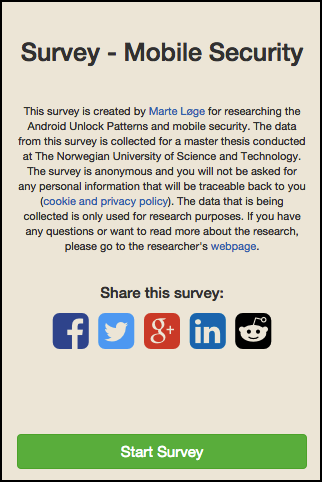
\includegraphics[scale=0.34]{pics/survey/start}
          \label{fig:startscreen}
        }
        \subfigure[ALP introduction]{
          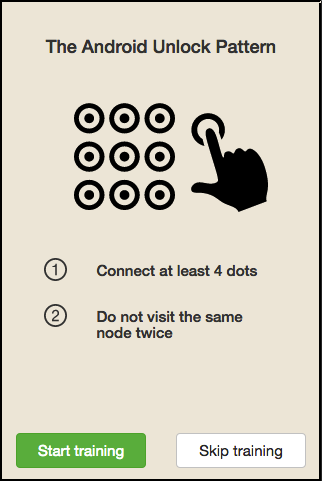
\includegraphics[scale=0.34]{pics/survey/rules}
          \label{fig:ALPintroduction}
        }
        \subfigure[Training mode]{
          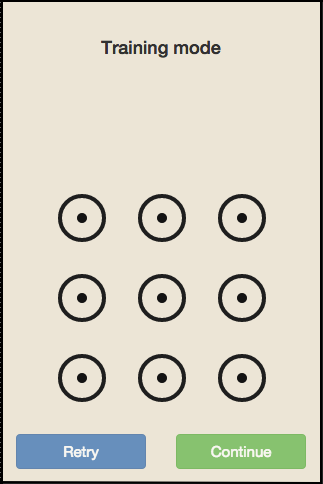
\includegraphics[scale=0.34]{pics/survey/training}
          \label{fig:trainingmode}
        }
        \caption{Survey screens}
        \label{fig:introductionviews}
      \end{figure}

    \subsubsection{Pattern creation}
      After introducing the research and the android pattern lock it is time to start collect the three main patterns for shopping account, smartphone, and banking account.
      The reason for dividing the pattern collection in three parts instead of just asking participants about a creating a pattern for smartphone is to put the patterns into context. 

      There will might be positive and negative effects by collecting three patterns instead of two. Looking at some of the possible negative outcomes is that people are not used to use android patterns in other contexts than the smartphone. Also asking people to create a pattern for a banking account can for someone be a scary situation and it is possible that some respondents will stop answering the survey. By asking the participants to create three instead of one pattern takes more time and it requires more attention and creativity from the participant. 

      It might be a situation that some people just create the same pattern for all pattern types, but that situation is hard to avoid. The decision to add three patterns instead of two is a preventive measure for avoiding data submitted by respondents just trying to finish the survey as soon as possible without thinking about what they are submitting, but will give more data giving a solid foundation for the analysis. 

      In this survey I chose to ask the participants to create a pattern for a shopping account, a smartphone and a banking account. The three types are selected after my subjective opinion of how people would categorize different situations in a security perspective. A known security situation, that is not related to computer security, is the problem of selected whether to drive a car or take an airplane. Statistically th airplane are safer, but many people would still take the car. I believe this situation can be transferred to computer security. The question is not the probability of being hurt, but rather the actual outcome of the situation when it occurs. A airplane crashing sound more dramatic than an car crashing. The outcome of being robbed from a banking account sound more dramatic than your shopping account being hacked. The problem with this is that the shopping account site might be insecure or should not be trusted, and as a predictable person you might use that password somewhere else. Looking at the bank, security is probably highly prioritized, so the probability of you being robbed would actually be very small. 
      %Folk har en rar måte å tenke på sikkerhet. Vi vil helst kjøre bil enn å ta fly feks. 

    \begin{figure}[H]
      \centering
      \subfigure[Draw pattern]{
        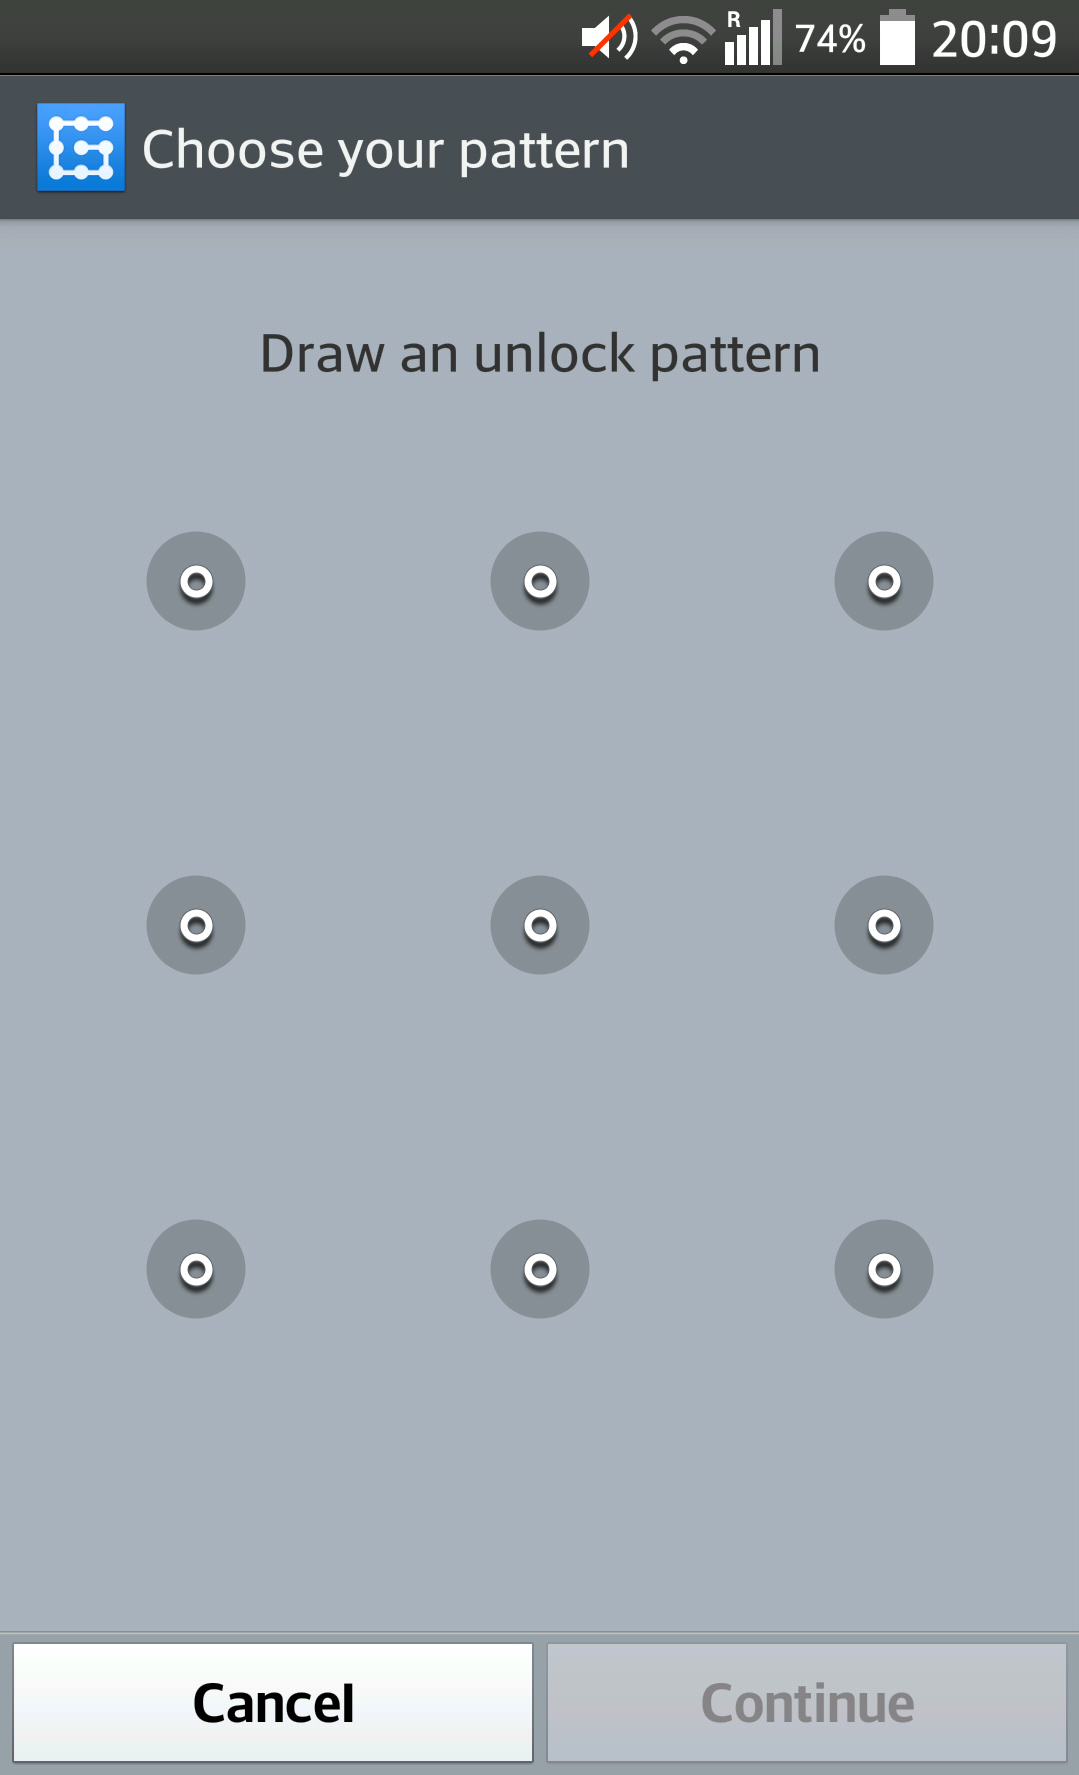
\includegraphics[scale=0.09]{pics/experiment/patternprocess3.png}
        \label{fig:drawpattern}
      }
      \subfigure[Pattern recorded]{
        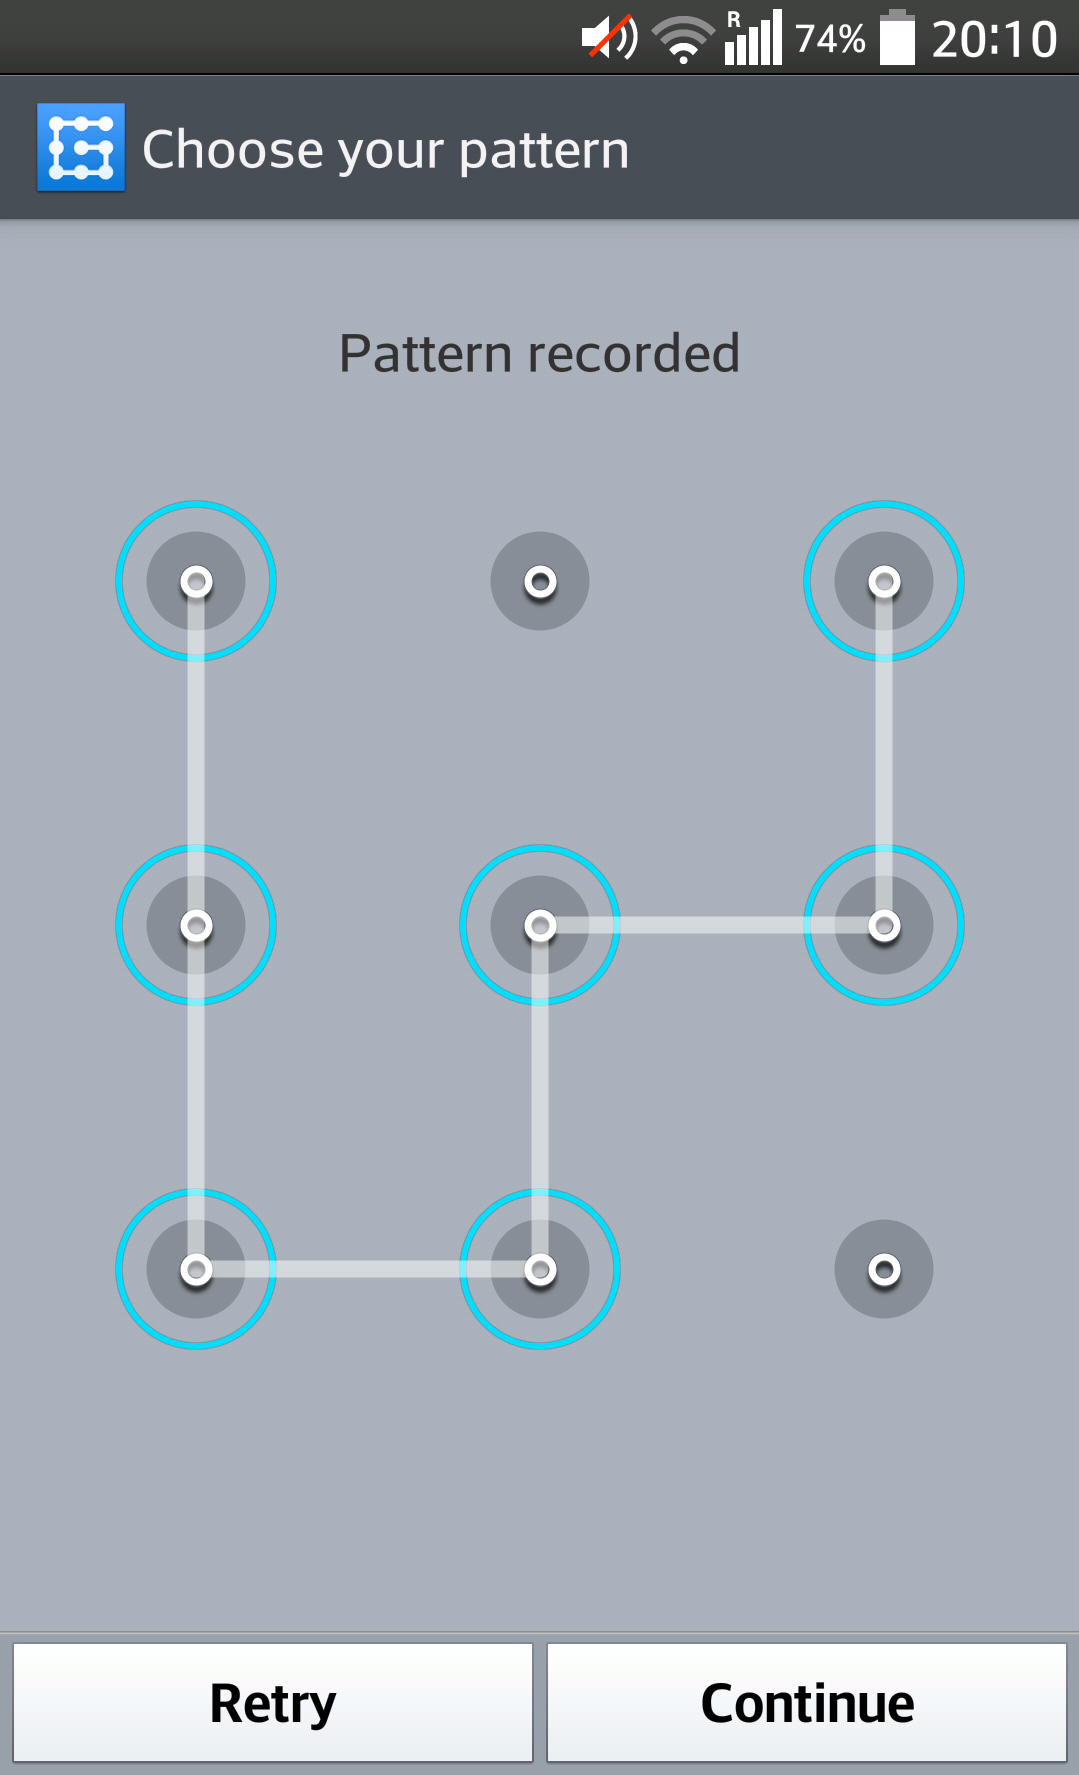
\includegraphics[scale=0.09]{pics/experiment/patternprocess4.png}
        \label{fig:patternrecorded}
      }\\
      \subfigure[Redraw pattern]{
        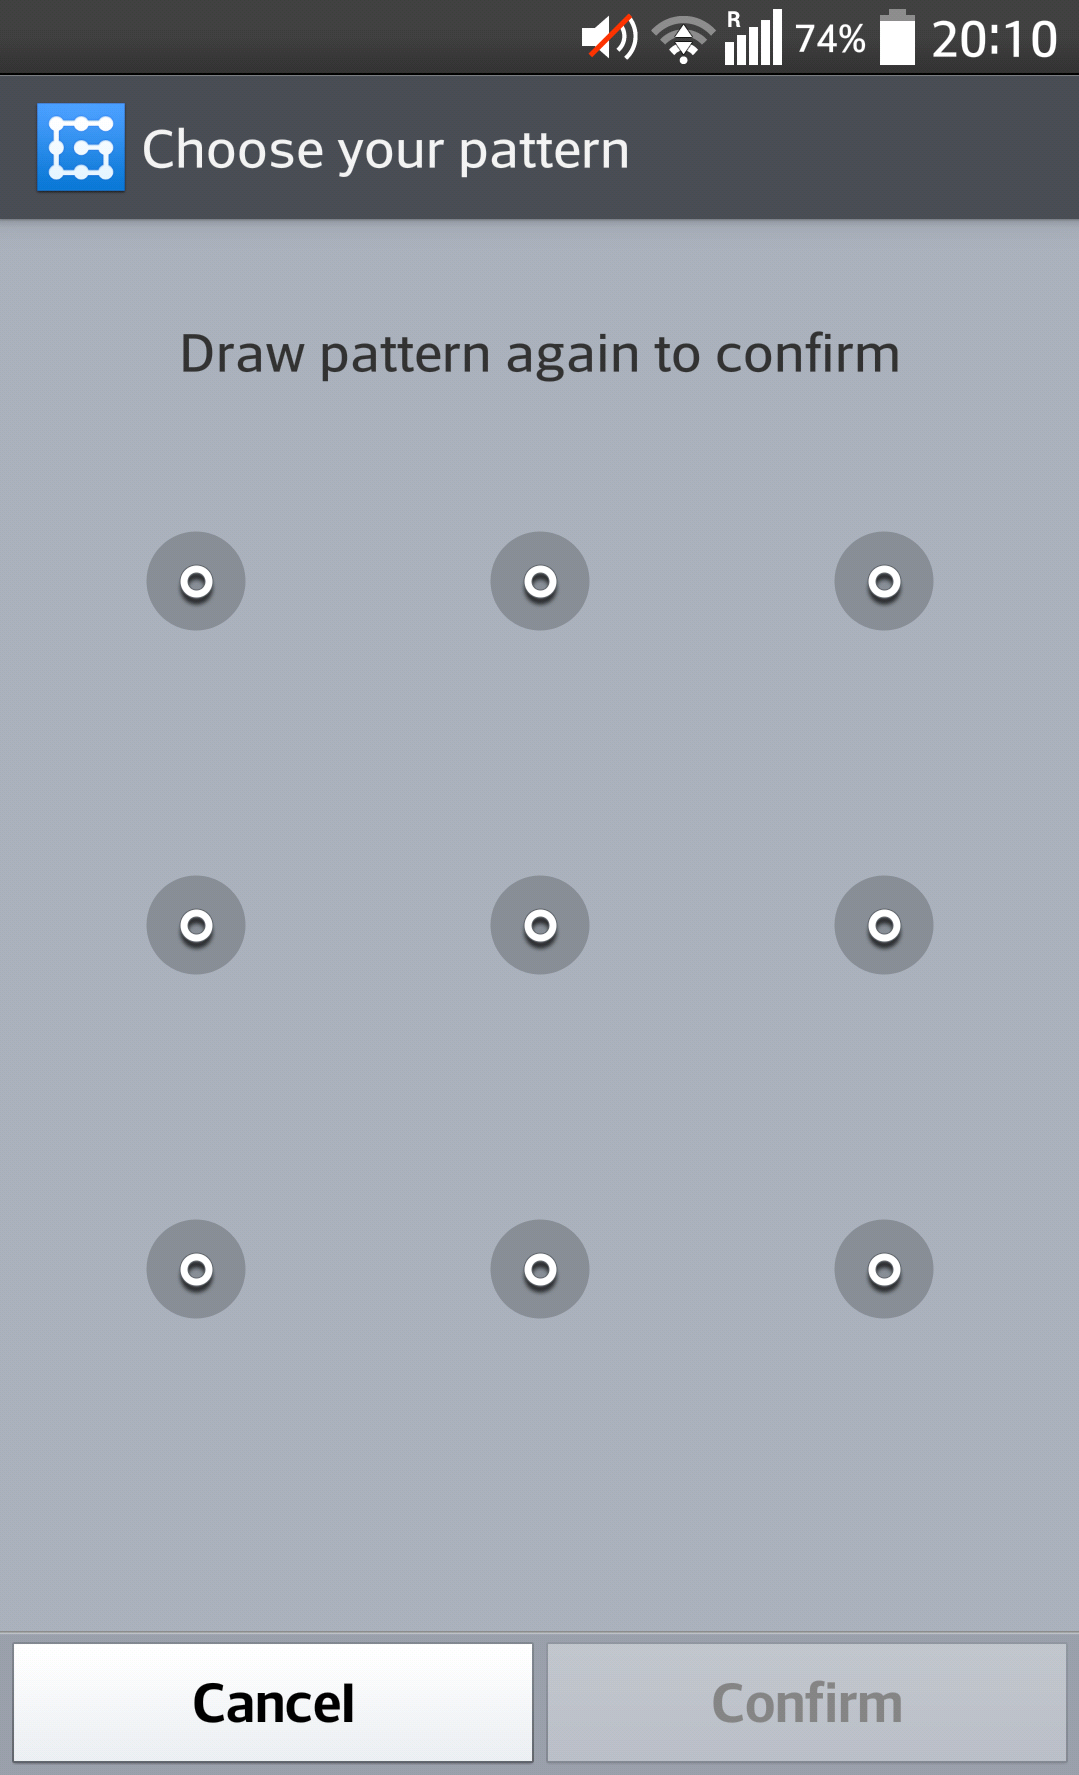
\includegraphics[scale=0.09]{pics/experiment/patternprocess5.png}
        \label{fig:redrawpattern}
      }
      \subfigure[Confirm new pattern]{
        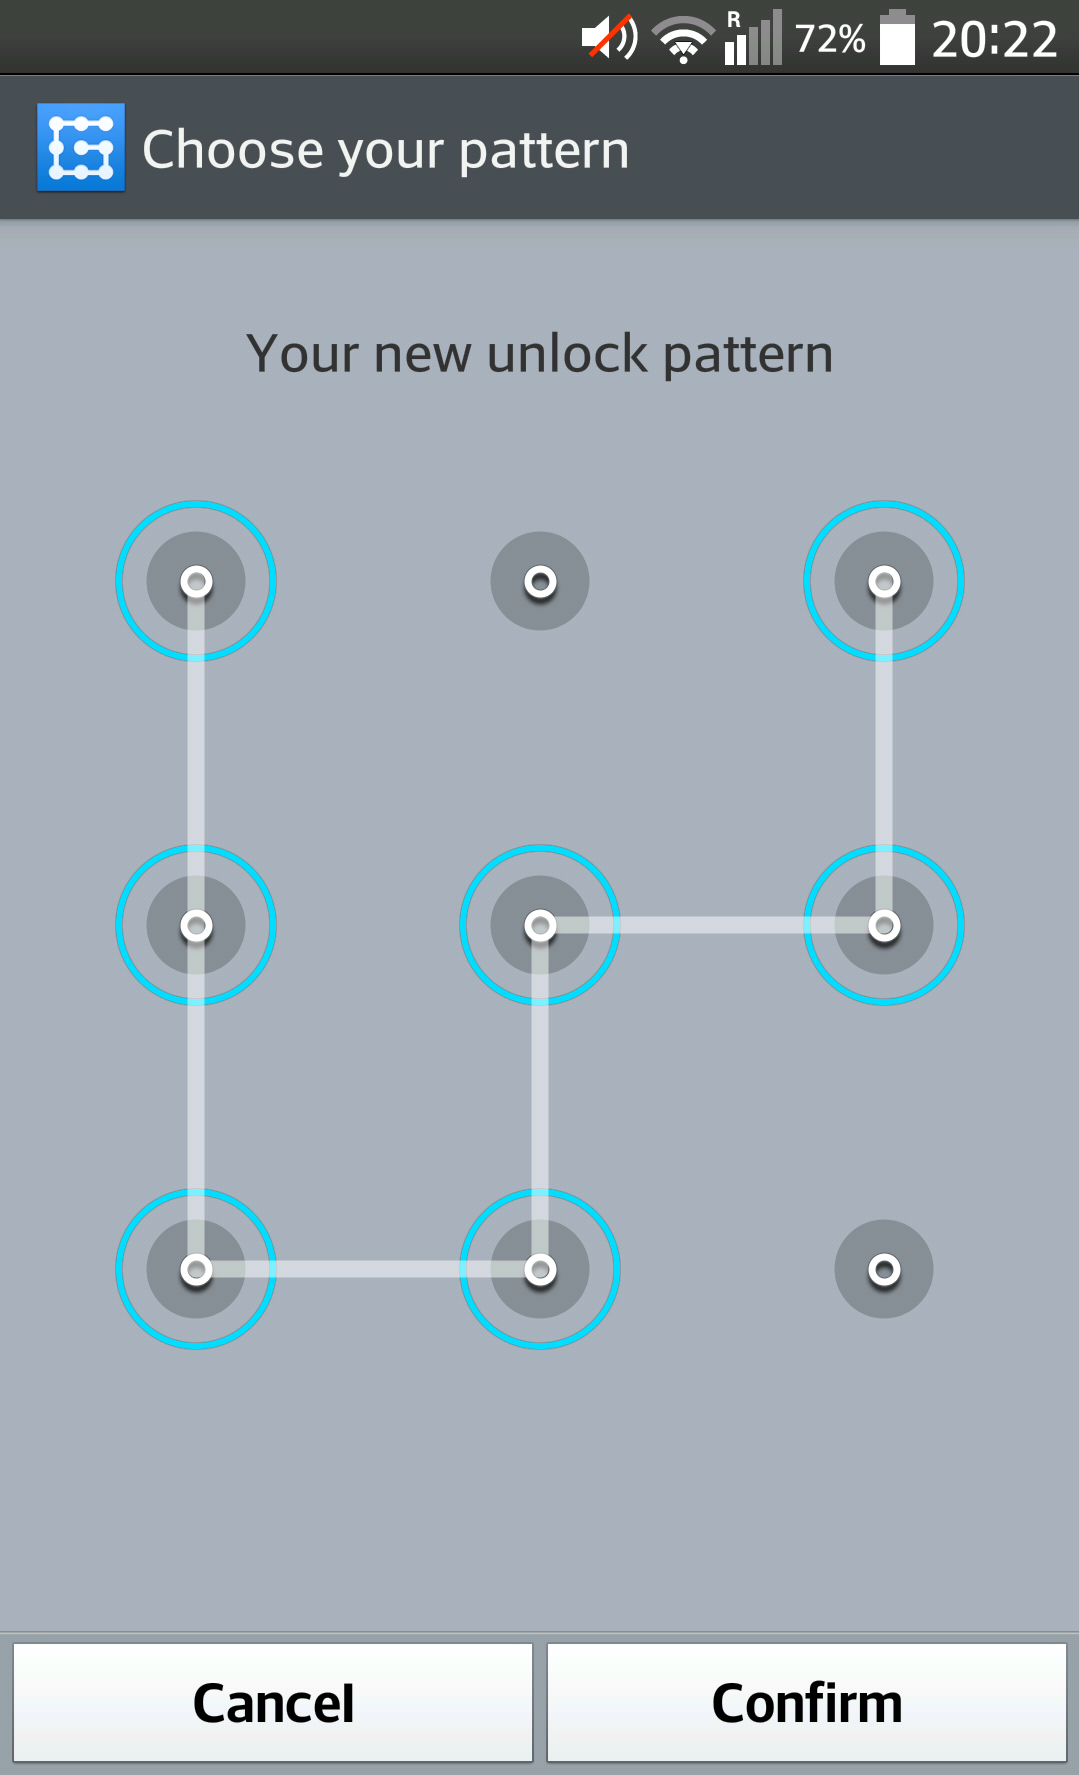
\includegraphics[scale=0.09]{pics/experiment/patternprocess1.png}
        \label{fig:confirmnewpattern}
      }
      \caption{The Android pattern creation process}
      \label{fig:androidpatterncreationprocess}
    \end{figure}

    When collecting the patterns it is desirable to copy the pattern creation process used by Android. The process consists of 2 steps: typing a pattern and retyping a pattern. Figure \ref{fig:drawpattern} is the first screen visualized to the user asking the user to draw a lock pattern. Figure \ref{fig:patternrecorded} shows the recorded pattern. Figure \ref{fig:redrawpattern} and Figure \ref{fig:confirmnewpattern} is the same process, but this time the user redraws the same pattern created in Figure \ref{fig:patternrecorded}.

    Figure \ref{fig:shoppingpattern}, \ref{fig:smartphonepattern}, and \ref{fig:bankpattern} are showing the three patterns to be created. When the user draws a pattern the participant have to follow the rules of the Android Unlock Pattern. If the pattern is too short there pattern will turn red and a error message will be shown as in Figure \ref{fig:patternlengthtooshort}. If a valid pattern is drawn, the dots will turn red and show a message saying that pattern was recorded as in Figure \ref{fig:validpatternrecorded}.

    

    \begin{figure}[H]
      \centering
      \subfigure[Introduction to patterns]{
        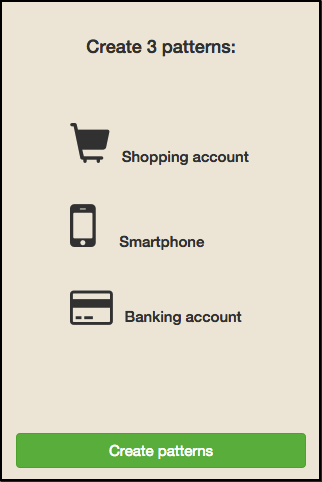
\includegraphics[scale=0.3]{pics/survey/pattern-introduction}
        \label{fig:introductiontopatterns}
      }
      \subfigure[Shopping pattern]{
        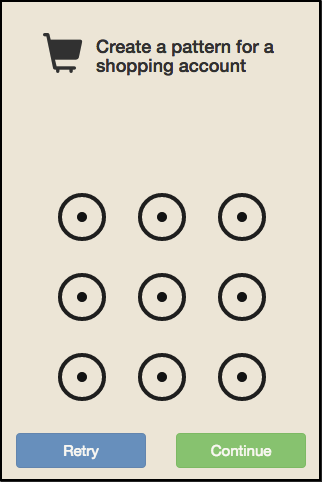
\includegraphics[scale=0.3]{pics/survey/shopping}
        \label{fig:shoppingpattern}
      }
      \subfigure[Smartphone pattern]{
        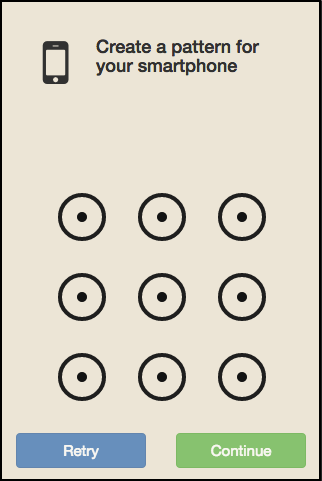
\includegraphics[scale=0.3]{pics/survey/smartphone}
        \label{fig:smartphonepattern}
      }
      \subfigure[Bank pattern]{
        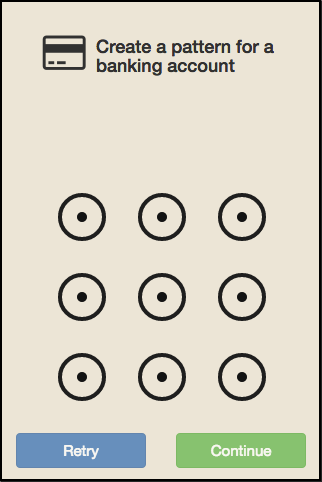
\includegraphics[scale=0.3]{pics/survey/bank}
        \label{fig:bankpattern}
      }
      \subfigure[Pattern length too short]{
        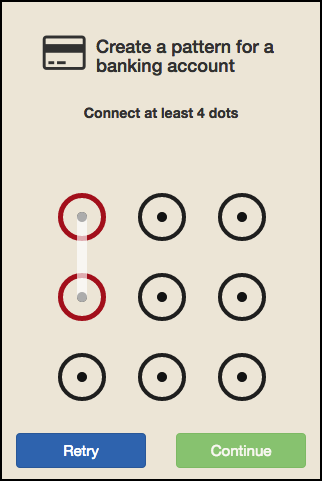
\includegraphics[scale=0.3]{pics/survey/not-valid-pattern-bank}
        \label{fig:patternlengthtooshort}
      }
      \subfigure[Valid pattern recorded]{
        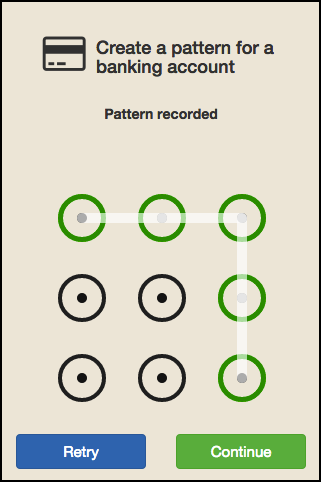
\includegraphics[scale=0.3]{pics/survey/pattern-recorded-bank}
        \label{fig:validpatternrecorded}
      }
      \subfigure[Retype pattern]{
        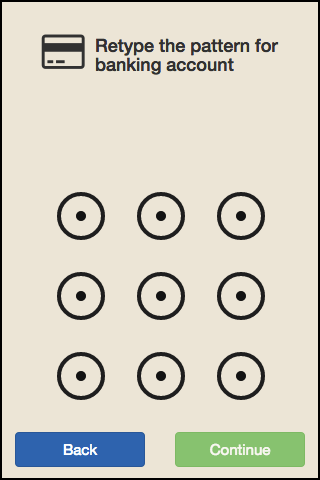
\includegraphics[scale=0.3]{pics/survey/retype-bank}
        \label{fig:retypepattern}
      }
      \subfigure[Retype wrong]{
        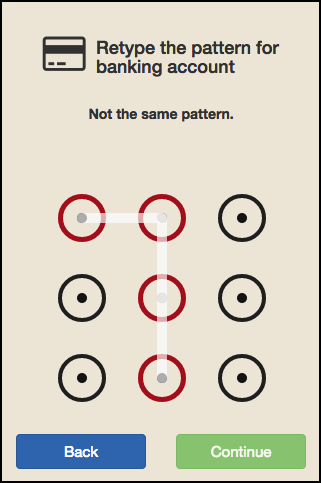
\includegraphics[scale=0.3]{pics/survey/not-valid-retype-bank}@
        \label{fig:retypewrong}
      }
      \subfigure[Retype correct]{
        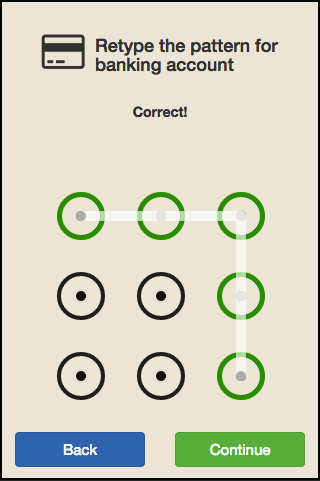
\includegraphics[scale=0.3]{pics/survey/retype-correct-bank}
        \label{fig:retypecorrect}
      }
      \caption{Survey - Create and retye patterns}
      \label{fig:createandretypepatterns}
    \end{figure}

    \begin{figure}[H]
      \centering
      \subfigure[Handsize]{
        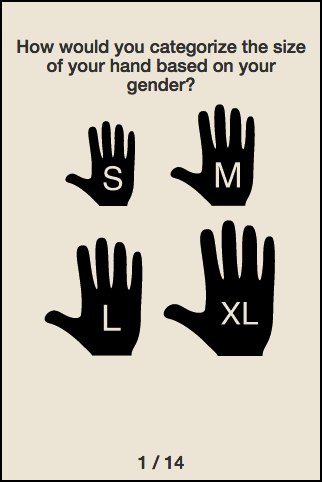
\includegraphics[scale=0.3]{pics/survey/handsize}
        \label{fig:handsizeview}
      }
      \subfigure[Handedness]{
        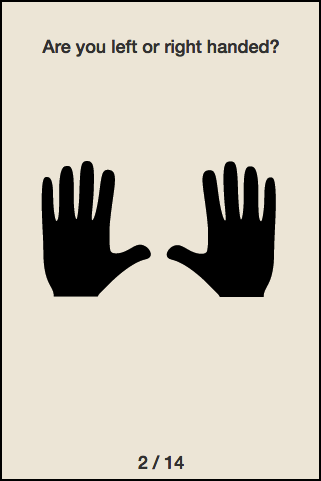
\includegraphics[scale=0.3]{pics/survey/handedness1}
        \label{fig:handednessview}
      }
      \subfigure[Screen size]{
        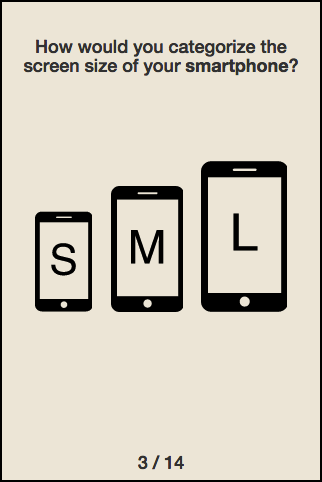
\includegraphics[scale=0.3]{pics/survey/screen}
        \label{fig:screensizeview}
      }
      \subfigure[Hand used when creating pattern]{
        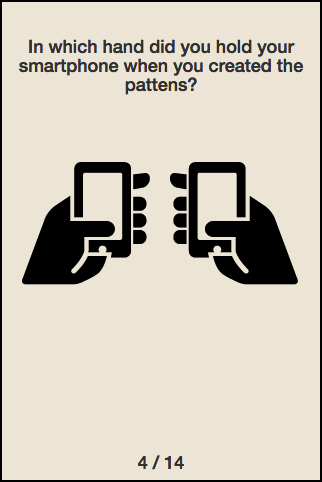
\includegraphics[scale=0.3]{pics/survey/handedness2}
        \label{fig:handusedview}
      }
      \subfigure[Finger used]{
        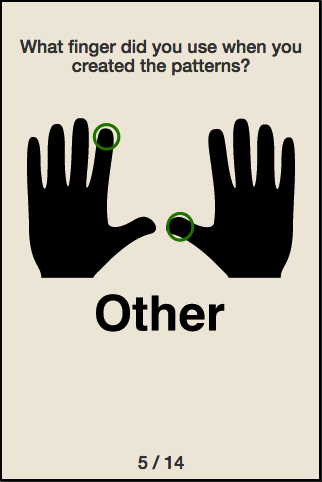
\includegraphics[scale=0.3]{pics/survey/finger}
        \label{fig:fingerusedview}
      }
      \subfigure[Reading/writing direction]{
        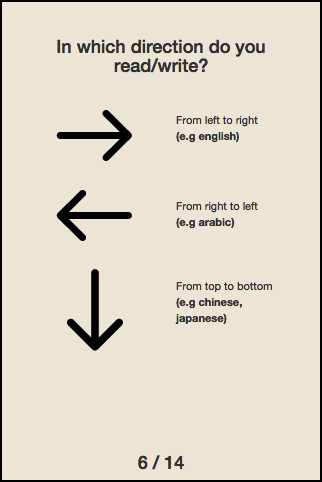
\includegraphics[scale=0.3]{pics/survey/reading}
        \label{fig:readingandwritingview}
      }
      \subfigure[Gender]{
        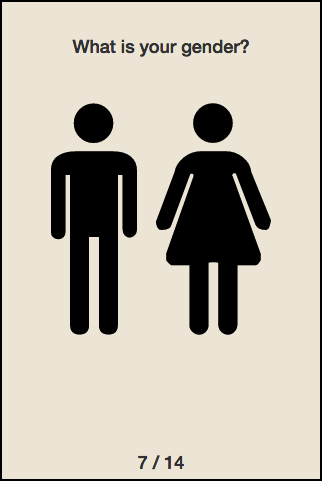
\includegraphics[scale=0.3]{pics/survey/gender}
        \label{fig:genderview}
      }
      \subfigure[Age]{
        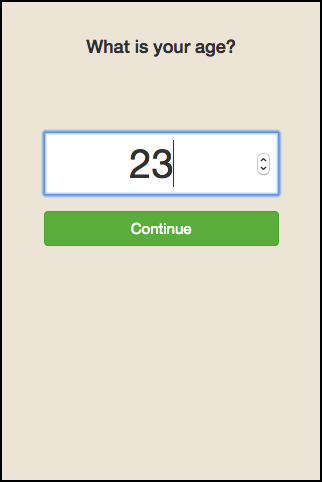
\includegraphics[scale=0.3]{pics/survey/age-2}
        \label{fig:ageview}
      }
      \caption{Survey - Questions}
      \label{fig:surveyquestoins}
    \end{figure}

    \begin{figure}[H]
      \centering
      \subfigure[Start screen]{
        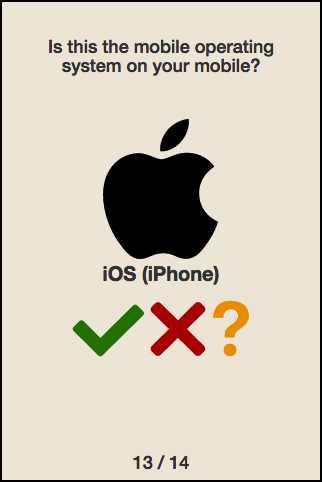
\includegraphics[scale=0.34]{pics/survey/ios}
      }
      \subfigure[ALP introduction]{
        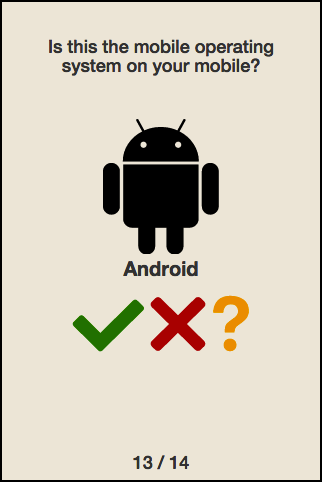
\includegraphics[scale=0.34]{pics/survey/android}
      }
      \subfigure[Training mode]{
        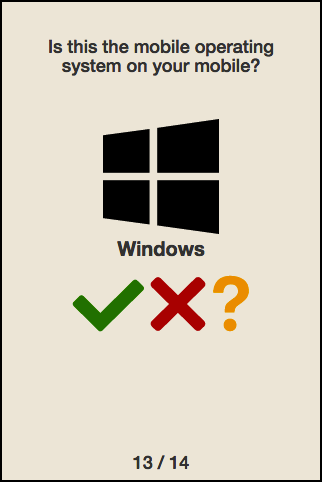
\includegraphics[scale=0.34]{pics/survey/windows}
      }
      \caption{Survey - Mobile OS}
    \end{figure}

    \begin{figure}[H]
      \centering
      \subfigure[Select icon]{
        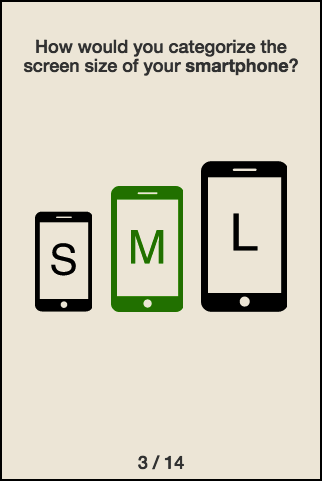
\includegraphics[scale=0.34]{pics/survey/icon-selected-1}
      }
      \subfigure[Icon fading out]{
        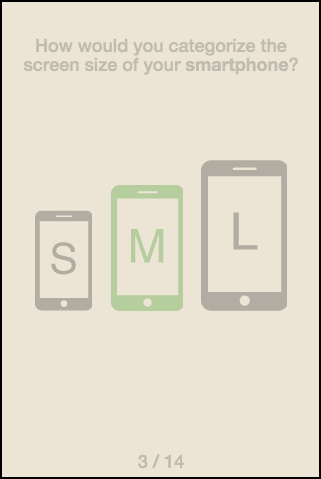
\includegraphics[scale=0.34]{pics/survey/icon-selected-3}
      }
      \subfigure[Icon faded out]{
        
\includegraphics[scale=0.34]{pics/survey/icon-selected-4}
      }
      \caption{Survey - Icon selecting effect}
    \end{figure}

\subsection{Technical Description of The Survey Application}

